
\documentclass[tikz,border=10pt]{standalone}

\usepackage{tikz}
\usetikzlibrary{trees,positioning,arrows.meta,shapes}

\begin{document}

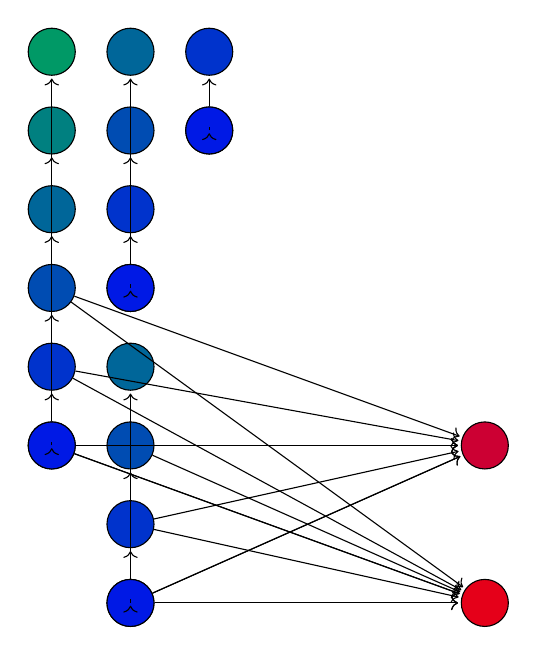
\begin{tikzpicture}[shorten >=1pt,->]
\tikzstyle{every pin}+=[fill=white!0,draw=black,thick,pin distance=50pt]
\tikzstyle{selected node}+=[ellipse,fill=red!24]
\tikzstyle{neuron}+=[circle,draw,minimum size=17pt,inner sep=0pt]
\tikzstyle{input neuron}+=[neuron, fill=green!50];
\tikzstyle{output neuron}+=[neuron, fill=blue!50];
\tikzstyle{hidden neuron}+=[neuron, fill=yellow!50];
\foreach \l [count=\i] in {4,6,4,2}{
    \pgfmathsetmacro{\offset}{0.5*(\l-1)}
    \node [hidden neuron/.try, fill=red!\i0!blue] (h\i-0) at ({-\offset}, 2*\i) {};
    \foreach [count=\j] \x in {1,...,\l} {
        \node [neuron/.try, fill=green!\j0!blue] (h\i-\j) at ({-\offset}, 2*\i - 1 + \j) {};
        \draw [->] (h\i-0) -- (h\i-\j);
    }
}
\foreach \i in {1,2}{
    \node [output neuron/.try, fill=blue!\i0!red] (o\i) at (3, 2*\i) {};
    \foreach \j in {0,...,3}{
        \draw [->] (h1-\j) -- (o\i);
        \draw [->] (h2-\j) -- (o\i);
    }
}
\end{tikzpicture}

\end{document}
